\chapter{Strängars rörelse i vätskor}

%\subsubsection{Strängrörelser inom cellen}
Aktinfilament är polymerer som utgör en viktig byggsten för cellens cytoskelett och transportväg för motorprotein vilka formar och bidrar till cellens utseende, dynamik och stadga. För att kunna ge en mer detaljerad beskrivning av dessa egenskaper är studien av enstaka aktinfilaments dynamik av stort intresse. I detta arbete har olika dynamiska egenskaper för aktinfilament studerats, både för filament som fluktuerar fritt i en vätska och filament instängda i en rektangulär kvasi-2D-mikrokanal -- alltså att kanalen har försumbart djup. Mikrokanalen är till för att simulera beteendet hos aktinfilament i cytoskelettet där det omges av andra filament och därmed har en begränsad möjlighet till rörelse.

Det här kapitlet börjar med en översikt över hur mikroskopidatan behandlas för att kunna användas i studien av strängarna. Därefter presenteras och undersöks en modell för fria strängröreler samt en modifikation av modellen som beskriver inneslutna strängar. Till sist beskrivs en undersökning av strängarnas egenmoder.

\section{Undersökt data}
Datan som analyseras för strängrörelse i vätska är sammma som Köster et~al.~\cite{Koster_etal2005,Koster_etal2007} använde och består av filmer av aktinfilament som tillåts röra sig i en vätska. Dessa strängar hade en längd kring 10--30\,\micro{m} och befann sig i kanaler av olika bredd. %\todo{Kanaler av olika bredd?Inte helt konsistent med stycket nedan}

Två typer av strängar studeras: fria strängar i breda kanaler och inneslutna strängar i en kvasi-2D-mikrokanal. Upplösning på filmerna är 10 bilder per sekund. Rörelsen utfördes till största del i två dimensioner då kanalernas djup var litet i förhållande till kanalernas och filamentens bredd.


\subsection{Polynomanpassning för strängarna} \label{sec:polynomanpassning}

\begin{figure}\centering
% GNUPLOT: LaTeX picture with Postscript
\begingroup
  \makeatletter
  \providecommand\color[2][]{%
    \GenericError{(gnuplot) \space\space\space\@spaces}{%
      Package color not loaded in conjunction with
      terminal option `colourtext'%
    }{See the gnuplot documentation for explanation.%
    }{Either use 'blacktext' in gnuplot or load the package
      color.sty in LaTeX.}%
    \renewcommand\color[2][]{}%
  }%
  \providecommand\includegraphics[2][]{%
    \GenericError{(gnuplot) \space\space\space\@spaces}{%
      Package graphicx or graphics not loaded%
    }{See the gnuplot documentation for explanation.%
    }{The gnuplot epslatex terminal needs graphicx.sty or graphics.sty.}%
    \renewcommand\includegraphics[2][]{}%
  }%
  \providecommand\rotatebox[2]{#2}%
  \@ifundefined{ifGPcolor}{%
    \newif\ifGPcolor
    \GPcolortrue
  }{}%
  \@ifundefined{ifGPblacktext}{%
    \newif\ifGPblacktext
    \GPblacktexttrue
  }{}%
  % define a \g@addto@macro without @ in the name:
  \let\gplgaddtomacro\g@addto@macro
  % define empty templates for all commands taking text:
  \gdef\gplbacktext{}%
  \gdef\gplfronttext{}%
  \makeatother
  \ifGPblacktext
    % no textcolor at all
    \def\colorrgb#1{}%
    \def\colorgray#1{}%
  \else
    % gray or color?
    \ifGPcolor
      \def\colorrgb#1{\color[rgb]{#1}}%
      \def\colorgray#1{\color[gray]{#1}}%
      \expandafter\def\csname LTw\endcsname{\color{white}}%
      \expandafter\def\csname LTb\endcsname{\color{black}}%
      \expandafter\def\csname LTa\endcsname{\color{black}}%
      \expandafter\def\csname LT0\endcsname{\color[rgb]{1,0,0}}%
      \expandafter\def\csname LT1\endcsname{\color[rgb]{0,1,0}}%
      \expandafter\def\csname LT2\endcsname{\color[rgb]{0,0,1}}%
      \expandafter\def\csname LT3\endcsname{\color[rgb]{1,0,1}}%
      \expandafter\def\csname LT4\endcsname{\color[rgb]{0,1,1}}%
      \expandafter\def\csname LT5\endcsname{\color[rgb]{1,1,0}}%
      \expandafter\def\csname LT6\endcsname{\color[rgb]{0,0,0}}%
      \expandafter\def\csname LT7\endcsname{\color[rgb]{1,0.3,0}}%
      \expandafter\def\csname LT8\endcsname{\color[rgb]{0.5,0.5,0.5}}%
    \else
      % gray
      \def\colorrgb#1{\color{black}}%
      \def\colorgray#1{\color[gray]{#1}}%
      \expandafter\def\csname LTw\endcsname{\color{white}}%
      \expandafter\def\csname LTb\endcsname{\color{black}}%
      \expandafter\def\csname LTa\endcsname{\color{black}}%
      \expandafter\def\csname LT0\endcsname{\color{black}}%
      \expandafter\def\csname LT1\endcsname{\color{black}}%
      \expandafter\def\csname LT2\endcsname{\color{black}}%
      \expandafter\def\csname LT3\endcsname{\color{black}}%
      \expandafter\def\csname LT4\endcsname{\color{black}}%
      \expandafter\def\csname LT5\endcsname{\color{black}}%
      \expandafter\def\csname LT6\endcsname{\color{black}}%
      \expandafter\def\csname LT7\endcsname{\color{black}}%
      \expandafter\def\csname LT8\endcsname{\color{black}}%
    \fi
  \fi
  \setlength{\unitlength}{0.0500bp}%
  \begin{picture}(6802.00,2834.00)%
    \gplgaddtomacro\gplbacktext{%
    }%
    \gplgaddtomacro\gplfronttext{%
      \csname LTb\endcsname%
      \put(3834,2352){\makebox(0,0)[r]{\strut{}Rådata}}%
      \csname LTb\endcsname%
      \put(3834,2132){\makebox(0,0)[r]{\strut{}Polynomanpassning}}%
      \csname LTb\endcsname%
      \put(3834,1912){\makebox(0,0)[r]{\strut{}Kubisk splineinterpolation}}%
    }%
    \gplbacktext
    \put(0,0){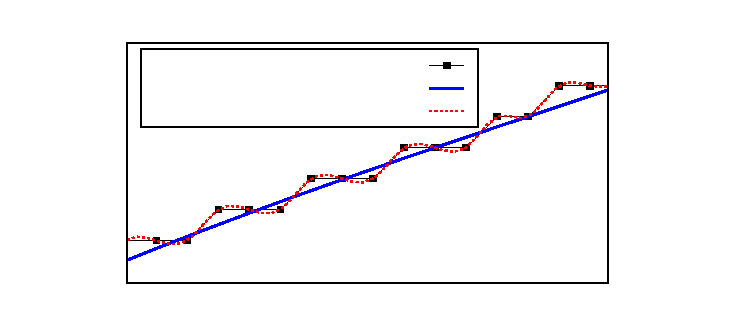
\includegraphics{strang_anpassning}}%
    \gplfronttext
  \end{picture}%
\endgroup

\caption{
Utdrag med pixelpositioner från en av strängarna tillsammans med polynomanpassningen som användes i denna studie samt en spline mellan pixlarna. Utdraget är bara av en mycket liten del av strängen för att enskilda pixlar ska synas.
Eftersom exempelvis tangent- och normalvektorer till strängarna är intressanta att studera behövs mjuka anpassningar till rådatan så att det går att derivera längs med strängen. 
}
\label{fig:strang_anpassning}
\end{figure}

Mätdatan för strängarna bestod vid varje tidpunkt av en matris med element motsvarande pixlarna på kameran. Datan var förbehandlad och strängen representerades som ett antal 1:or i en annars tom matris. 
För att kunna arbeta effektivt med strängarna behövs dock någon form av anpassning till dessa ''pixlar''. Bland annat behövs mjuka anpassningar för att kunna ta fram tangent- och normalvektorer i en godtycklig punkt längs med strängen. I \figref{fig:strang_anpassning} visas ett litet utdrag av en sträng med pixlepositioner och anpassningar. 

För att kunna göra en anpassning behövs först och främst en parameter som kan användas för att anpassa mot. 
Strängens position i varje tidsögonblick parametriserades med en normerad båglängdsparametern $s\in[0,1]$. Alltså att $s$ svarar mot hur stor andel av strängens längd som ligger bakom punkten svarande mot det $s$-värdet. 
För att i MATLAB bilda båglängsdparametern sorterades först punkterna i en ordnad följd längs med strängen. Efter detta uppskattades hur långt längs med strängen varje pixel på strängen låg. Detta gjordes genom att ackumulera längderna på de förbindande linjerna mellan varje pixel. På så sätt erhålls ett $s$-värde för varje pixel och nu kan en anpassnings göras av pixlarnas $x$- och $y$-koordinaterna mot $s$.

I den här studien valde vi att anpassa positionerna i varje tidpunkt med ett polynom av grad $20$ för vardera $x_t$ och $y_t$ enligt
\begin{equation}\label{eq:anpassning}
x_t(s) = \sum_{n=0}^{20} a_n^{(t)} \,s^n,
\end{equation}
där koefficienterna $a_n^{(t)}$ anpassades med hjälp av MATLABs \texttt{polyfit}-funktion till varje pixels position och $s$-värde. På samma sätt kunde även ett polynom för $y$ anpassas. Att det skulle krävas ett 20-gradspolynom för att följa strängen syns inte i \figref{fig:strang_anpassning} på grund av att figuren bara visar en mycket liten del av strängen. Graden behövde dock vara så hög för att de anpassade polynomen skulle kunna följa strängen bra längs med hela strängens längd. 

Sedan får inte graden väljas mycket högre än cirka 20 för att inte få med andra artefakter från polynomanpassning såsom en variant av Runges fenomen\cite{Gustafsson_LaNa}. Alltså att polynomet börja svänga kraftigt för att exakt gå igenom alla punkter som det ska anpassas till. Detta är i regel ett problem för interpolationer och inte anpassningar, men om gradtalet väljs ungefär lika stort som antalet punkter som ska anpassas så tenderar anpassningen att bli som en interpolation.


\subsubsection{Alternativa metoder för att anpassa en kurva till strängdata}

\figref{fig:strang_anpassning} visar också en kubisk splineinterpolation som också är ett sätt som använts för att anpassa en kurva till strängen~\cite{Koster_etal2005,Koster_etal2007}. Dock anser vi att beteendet som splineinterpolationen uppvisar i \figref{fig:strang_anpassning} inte speglar den verkliga strängens form. Det är inte särskilt troligt att den verkliga strängen helt skulle följa varje pixel, utan det är mer rimligt att den verkliga strängen följer en sorts medelposition av pixlarna. 

En sak som ytterligare talar för att splineinterpolation inte är en optimal anpassningsmetod är svängningarna\footnotemark{} som syns i \figref{fig:strang_anpassning} mellan pixlarna. Dessa svängningar är över längdskalor som är mindre än mikroskopets upplösning. Det är alltså inte motiverat att använda sig av en metod som ger information som inte går att observera. 
\footnotetext{Dessa svängningar är dock inte ett exempel på Runges fenomen. Eftersom en kubisk spline är flera olika tredjegradspolynom fås inte beteendet från ett höggradit polynom\cite{Gustafsson_LaNa}. }


\subsection{Mäta avstånd från jämviktsläge}

\begin{figure}
\centering
\resizebox{0.8\textwidth}{!}{
    \input{bilder/strangar/transv_avst.pdf_t}
}
\caption{Schematisk skiss av hur transversella avståndet från medelsträngen mäts. I varje tidpunkt jämförs medelsträngens position, $\mathbf{r}_0(s)$, med den momentana strängens position, $\mathbf{r}(s, t)$, för samma $s$-värde -- $s$ är en parameter som motsvarar en viss sträcka längs med strängen. För att få ett avståndsmått som kan växla tecken undersöks projiceringen av skillnaden i ortsvektor på medelsträngens normalvektor. 
}
\label{fig:transv_avst}
\end{figure}

I denna rapport har strängens translationsrörelse till stor del försummats genom att i varje tidpunkt placerat strängens masscentrum i origo. Givet detta är det intressant att studera huruvida strängarna fluktuerar kring något jämviktsläge. En uppskattning av jämviktsläget $\mathbf{r}_0(s)$ tas fram genom att beräkna medelvärdeskurvan som representerar strängrörelsen. 

Från detta jämviktsläge har det transversella avståndet beräknats enligt 
\begin{equation}
A_s(t) = \mathbf{n}_0(s)\cdot\Big(\mathbf{r}(s,t)-\mathbf{r}_0(s)\Big),
\end{equation}
där $\mathbf{n}_0(s)$ är en normerad normalvektor till strängens jämviktsläge samt $\mathbf{r}(s,t)$ och $\mathbf{r}_0(s)$ är ortsvektorerna för momentansträngen respektive medelsträngen. Avståndet $A_t(s)$ motsvarar alltså projektionen av $(\mathbf{r}(s,t)-\mathbf{r}_0(s))$ på normalvektorn. Detta 
illustreras i \figref{fig:transv_avst}.








\section{Modeller för strängrörelser}

Aktinfilamenten precis som tidigare studerade partiklar påverkas av diffusionsprocessen inuti celler och således krävs stokastiska modeller för att beskriva rörelsen. En vanligt använd modell inom polymerfysiken är Worm Like Chain-modellen som beskrivs nedan. Vidare studeras en annan, fenomenologisk modell baserad på en langevinekvation. 



\subsection{Worm Like Chain-model}

Worm like chain modellen \cite{Milstein2013} (WLC) är en modell som ämnar beskriva fluktuationerna hos en semi-flexibel polymer. I modellen antas att polymeren är helt oelastisk, enbart påverkas av termiskt brus och styv på små längdskalor. Om polymeren fluktuerar fritt %utan att vara instängd i en mikrokanal 
ges en minimalistisk WLC beskrivning av att filamentets fluktuationer regleras av böjningsenergin. För en polymer med $N$ segment vardera med riktning \textbf{r}$_i$ och längd $\abs{r_{i}}=l$ samt polymerens böjstyvhet $\kappa$ ges böjningsenergin av
\begin{equation}
    H = -\kappa\sum_{i=1}^{N}\textbf{r}_{i}\cdot \textbf{r}_{i+1}.
\end{equation}
Maximalt bidrag till energin från två på varandra följande segment fås alltså om dessa har antiparallell riktning. Givet identiteten $\textbf{r}_{i}\cdot\textbf{r}_{i+1}=(2l^2-(\textbf{r}_{i+1}-\textbf{r}_{i})^2)/2$ kan summan skrivas om som en integral i gränsen då $N \to \infty$, $\kappa\to\infty$, $l \to 0$ men där produkten $\kappa l=\xi$ är finit som 
\begin{equation}\label{böj}
    H=\frac{\xi}{2}\int_{0}^{L}\!\dd{s}\,(\partial_{s}\textbf{t}(s))^2,
\end{equation}
där $\textbf{t}(s)$ är enhetstangentvektorn längs polymeren parametriserad med båglängden. Detta är den kontinuerliga WLC modellen \cite{Fixman_WLC1973} vilket ger en bra approximation av en polymer där längden av enskilda molekyler kan försummas. Korrelationen mellan två tangentvektorer medelvärdsbildat över tid ges av \cite{Landau1958}:
\begin{equation}
\ev{\textbf{t}(s)\textbf{t}(s+\Delta s)}=\ee^{-\frac{\abs{\Delta s}}{2L_{p}}},
\end{equation}
där $L_{p}=\frac{\xi}{k_{B}T}$ är kvoten mellan styvheten hos polymeren och termiska energin hos fluiden. Denna kallas \emph{persistence length} och ger ett mått på hur snabbt tangentkorrelationen avtar längs polymeren. I fallet då $\nicefrac{L_{p}}{L}>1$ sägs polymeren vara styv. 
För att öka noggrannheten kan även ett rumsligt medelvärde tas över tangentkorrelationerna, låt denna betecknas med ett heldraget streck. Tangentkorrelationen beror då inte längre av var på strängen korrelationen tas utan bara på avståndet mellan tangentvektorerna, $\Delta s$, och defineras som
\begin{equation}
\label{tangkorr}
    \ev{\cos\theta(\Delta s)}\equiv\overline{\ev{\mathbf{t}(s)\mathbf{t}(s+\Delta s)}}.
\end{equation}
Denna minimalistiska WLC modell förutspår alltså tangentkorrelationens utseende utifrån antagandet att strängen tillåts fluktuera fritt.



\subsubsection{Resultat -- mikrokanalen påverkar strängens tangentkorrelation}



För att undersöka hurvida mikrokanalen påverkar strängen beräknas tangentkorrelation enligt \eqref{tangkorr} för både ''fria'' samt inneslutna strängar. \todo[color=olive]{fixa figur på tangentkorrelation för sträng 1 samt 3.}I figur .. ses tangentkorrelationer för de olika proverna plottade med anpassade potensamband i $\Delta s$. Det ses att en sträng påverkas av en mindre mikrokanal då dess tangentkorrelation upplevs mer ihärdig. Persistence length fås för strängarna som \todo[color=olive]{kontrollera dessa}.. respektive .. . Eftersom strängarna i de olika proverna är snarlika aktinfilament, vars enda signifikanta skillnad är båglängd, tolkas skillnaden i persistence length som ett mått på hur en strängs möjlighet att fluktuera begränsas av mikrokanalen. 



\subsection{WLC-modell för sträng i mikrokanal}
\label{WLCkanal}


En mer sofistikerad modell kan konstrueras med avseende på mikrokanalens egenskaper och dess dynamik. Då interaktionen mellan strängen och kanalens väggar beskrivs som rent sterisk \cite{Koster_etal2007} kan denna approximeras med en parabolisk potential. Inför därför kraften $F \propto A(s)$ där $A(s)$ svarar mot strängens vinkelräta avstånd från centrum av kanalen. Potentiella energi med avseende på dessa avvikelser fås som
\begin{equation}
    H_{pot}=\int_{0}^{L} \!\dd{s} \, [\gamma A(s)^2],
\end{equation}
där $\gamma$ är en positiv konstant vilket avger styrkan hos potentialen. 

Då tangentvektorn till strängen kan defineras som $\mathbf{t}(s)=\partial_sA(s)$, adderas denna energi till den tidigare härledda hamiltonianen enligt

\begin{equation}
\label{Htot}
    H_{tot}=\int_{0}^{L}\!\dd{s}\,[\xi\partial_{s}^{2}A(s)^2 + \gamma A(s)^2],
\end{equation}
där första termen i integranden svarar mot energin enligt den tidigare modellen \eqref{böj}.

Hamiltonianen ger nu en modell av den kraft vilket kan tänkas verka på en sträng i en mikrokanal. Det ses att potentiella energin för strängen minimeras i fallet då denna är rak och fixerad längs kanalens centrum. Alltså återställer kraften eventuella avvikelser från jämviktsläget. Då avvikelserna uppstår på grund av termiska fluktuationer, vilka antas vara stokastiska, kan som tidigare i avsnitt~\ref{sec:brown} systemet betraktas med en langevinekvation. Då strängens intrinsiska tröghet, svarandes mot högre ordningens tidsderivata, försummas fås\cite{PhysRevE.60.4671}
\todo{jobba på övergången}

\begin{equation}
\label{mans}
    \partial_{t}A(t,s)=-\gamma A(t,s)+\xi \partial_{s}^{2}A(t,s)+\sigma \partial_{t}W(t,s).
\end{equation}
Fluktuationerna approximeras med termen $W(t,s)$, ett stokastiskt vitt brus vars intensitet är proportionellt mot reella talet $\sigma>0$. Notera hur langevinekvationen även beskriver tidsutveckling av systemet.

\todo{eget kapitel? ev. flytta ner beräkningarna i apendix}

Definera fouriertransformation som 
\begin{equation}
    \hat{A}(t,k)=\int_{-\infty}^{\infty}\!\dd{s}\, A(t,s)\ee^{-\ii sk}
\end{equation}
Genom fouriertransformation av \eqref{mans} fås en ordinär stokastisk differentialekvation av första ordningen
\begin{equation}
        \partial_{t}\hat{A}(t,k)=-\left(\gamma+\xi k^2\right)\hat{A}(t,k)+\sigma \partial_{t}\hat{W}(t,k).
\end{equation}
I fallet då $\gamma+\xi k^2=\zeta$ ses det att denna ekvation är ekvivalent med \eqref{eq:Brownian_SDE} vars lösning är känd. Vidare kan kovariansen formuleras likt \eqref{Brownian_korr} det fås att
%\begin{equation}
%        \hat{A}(t,s)=\ee^{-(\gamma+\alpha s^2)t}\left(\hat{A}(0,s)+\sigma\int_{0}^{t}\dd\tau \ee^{(\gamma+\alpha s^2)\tau}\partial_{t}\hat{W}(\tau,z)\right)
%\end{equation}
%Tvåpunktskorrelationen för den fouriertransformerade stokastiska variabeln $\hat{A}(t,s)$ kan då beräknas till
\begin{equation}\label{jobbig}
\begin{aligned}
    \ev{\hat{A}(t,k)\hat{A}(t',k')} =& \ev{\hat{A}(0,k)\hat{A}(0,k')} \ee^{-(\gamma+\xi k^2)(t+t')}\\ 
    &+ \sigma^2 \int_{0}^{t}\int_{0}^{t'}\!\dd\tau\dd\tau' \ee^{(\gamma+\xi k^2)(\tau+\tau')} \ev{\partial_{t}\hat{W}(\tau,k)\partial_{t}\hat{W}(\tau',k')}.
\end{aligned}
\end{equation}
Integralen i \eqref{jobbig} beror på vitt brus i fourierrummet $\hat{W}(t,k)$. Denna beräknas rakt av genom fouriertransformation av \eqref{eq:white_noise}, vilket ger
\begin{equation}
    \ev{\partial_{t}\hat{W}(t,k)\partial_{t}\hat{W}(t',k')}=\delta(t-t')\delta(k+k').
\end{equation}
Insättning av detta resultat i \eqref{jobbig} samtidigt som ekvationen betraktas i gränsen då $t,t'\rightarrow\infty$ medan $\Delta t=\abs{t-t'}$ hålls finit erhålls
%\begin{equation}\label{jobbig}
%     \ev{\hat{A}(t,s)\hat{A}(t',s')}=\sigma^2\int_{0}^{t}\int_{0}^{t'}\dd\tau\dd\tau'\ee^{(\gamma+\alpha s^2)(\tau+\tau')}\ev{\partial_{t}\hat{W}(\tau,s)\partial_{t}\hat{W}(\tau',s')}.
%\end{equation}

%Då termiska bruset antas vara brownskt definieras det av följande tvåpunktskorrelation
%\begin{equation}\label{brus}
%    \ev{\partial_{t}W(t,z)\partial_{t}W(t',z')}=\delta(t- t')\delta(z-z')
%\end{equation}
%Fouriertransformation av \eqref{brus} ger \todo{ekvation 4.13+4.14 kanske kan skippas om man vill minska antal ekvationer.}
%\begin{equation}
%    \ev{\partial_{t}\hat{W}(t,s)\partial_{t}\hat{W}(t',s')}=\int_{-\infty}^{\infty}\int_{-\infty}^{\infty}\dd z \dd z'\ev{\partial_{t}W(t,z)\partial_{t}W(t',z')}\ee^{-izs}\ee^{-iz's'}
%\end{equation}
%\begin{equation}\label{fourbrus}
%    \ev{\partial_{t}\hat{W}(t,s)\partial_{t}\hat{W}(t',s')}=\delta(t-t')\int_{-\infty}^{\infty}\int_{-\infty}^{\infty}\dd z \dd z'\delta(z-z')\ee^{-i(sz+s'z')}=\delta(t-t')\delta(s+s')
%\end{equation}
\begin{equation}
    \ev{\hat{A}(t,k)\hat{A}(t',k')}=\frac{\sigma^2}{2(\gamma+\xi k^2)}\delta(k+k')\ee^{(\gamma+\xi k^2)\abs{t-t'}}.
\end{equation}
Slutligen återfås kovariansen för de rumsliga variblerna $s$,$s'$ genom invers fouriertransform
\begin{equation}
\label{2korr}
    \ev{A(t,s)A(t',s')}=\frac{\sigma^2}{(2\pi)^2\sqrt{\gamma\xi}}\int_{-\infty}^{\infty}\!\dd{p} \frac{\exp[-(1+p^2)\gamma \abs{t-t'}+\ii p\sqrt{\frac{\gamma}{\xi}}(s-s')]}{1+p^2},
\end{equation}
där variabeln $p$ är en hjälpvariabel definerad som $\frac{dp}{dk}=\sqrt{\frac{\xi}{\gamma}}$. 

Då kovariansen beror på differensen mellan variablerna $\Delta t=t-t'$ samt $\Delta s=s-s'$ är denna translationsinvariant. Det kan visas då för en godtycklig förflyttning i tiden $\delta{t}$ fås att $\ev{A(t,s)A(t',s')}=\ev{A(t+\delta t,s)A(t'+\delta t,s')}$. Därmed kan tvåpunktkorrelationen defineras som
\begin{equation}
    c(\Delta t,\Delta s)=\frac{\ev{A(\Delta t,\Delta s)A(0,0)}}{\ev{A(0,0)^2}}.
\end{equation}
Tolkningen av tvåpunktskorrelationen är att ge mått på hur snabbt avvikelser från strängens jämviktsläge skingras med tid samt avstånd på strängen. Givet data från strängar i mikrokanaler kan tvåpunktskorrelationen beräknas numeriskt och de fysikaliska parametrarna $\xi,\gamma,\sigma$ kan bestämmas. 

Tvåpunktskorrelationen kan även betraktas i två specialfall; då $\Delta t=0$, vilket likt den minimalisktiska WLC modellen svarar mot korrelation längs strängen, samt då $\Delta s=0$, vilket ger temporal korrelation. För båda fallen kan \eqref{2korr} lösas analytiskt, korrelationen längs strängen ges av
\begin{equation}
\ev{A(s)A(s')}=\exp(-\sqrt{\frac{\gamma}{\xi}}\abs{\Delta s}).
\end{equation}
Motsvarande ''persistence length'' för en sträng i en mikrokanal fås då som $L_{p}=\sqrt{\frac{\xi}{\gamma}}$.
Temporala korrelationen ges av
\begin{equation}
    \ev{A(t)A(t')}=erfc(\sqrt{\Delta t}),
\end{equation}
där $erfc(.)$ är \emph{complementary error function} definerad som $erfc(x)=\frac{2}{\sqrt{\pi}}\int_{x}^{\infty}\ee^{-y^2}\dd y$.


\subsubsection{Resultat -- ''tvåpunktskorrelation''}



\subsection{Egenmoder}
\todo{namn?}

Ett vanligt sätt att studera svängningar är att dela upp dem i egenmoder. Genom en linjärkombination av dessa egenmoder kan en godtycklig svängning representeras. Anledningen till att det är intressant att studera egenmoder är på grund av att de är oberoende av varandra. Precis som svängningen på en gitarrsträng kan strängens svängningar i cellen eventuellt representeras som en linjärkombination av dess egenmoder. 
\todo[color=olive]{flyttade runt ett par stycken, se till att övergången här är bra }
Återigen betrakta \eqref{mans}, då denna modell beskriver strängens svängningar kan det tänkas att dess lösningar kan uttryckas i en sådan linjärkombination. Alltså att positionsvektorn kan utvecklas i en bas av egenmoder
\begin{equation}
    A(t,s)=\sum_{n=1}^{\infty}a_{n}(t)\psi_{n}(s),
\end{equation}
där $a_{n}(t)$ är egenvärdet till respektive egenmod $\psi_{n}(s)$. Värdet på $a_{n}(t)$ svarar mot egenmodens amplitud vilket ansätts vara tidsberoende. Insättning i \eqref{mans} ger följande differentialekvation
\begin{equation}\label{egenvard}
    \sum_{n=1}^{\infty}\partial_{t}a_{n}(t)\psi_{n}(s)=\sum_{n=1}^{\infty}a_{n}(t)[\xi\partial_{s}^{2}-\gamma]\psi_{n}(s)+\sigma\partial_{t}W(t,s).
\end{equation}
Summanden i högerledet svarar mot en operator verkandes på moderna. Ansätt nu $\psi_{n}(s)$ att vara egenvektorer till operatorn, alltså att
\begin{equation}
    [\xi\partial_{s}^{2}-\gamma]\psi_{n}(s)=\lambda_{n}\psi_{n}(s),
\end{equation}
där $\lambda_{n}$ svarar mot egenvektorernas egenvärden till operatorn vilket antas vara tidsoberoende. Lösningar till denna egenvärdesekvation ges av de trigonometriska funktionerna, dock eftersträvas enbart lösningar vilket samtidigt spänner upp en möjlig bas till strängarnas svängningar. Då strängarnas ändar inte är fixa förkastas \emph{sinus}-delen av lösningen och moderna fås som \cite{PhysRevE.60.4671} $\psi_{n}(s)=\cos({\frac{n\pi}{L}s})$. Insättning av denna i \eqref{egenvard} reducerar återigen ekvationen till en ODE 
\begin{equation}
    \sum_{n=1}^{\infty}[\partial_{t}a_{n}(t)+\lambda a_{n}(t)]\psi_{n}(s)=\sigma\partial_{t}W(t,s).
\end{equation}
Medelvärdesbildas ekvationen över tid fås högerledet som $\ev{\sigma\partial_{t}W(t,s)}=0$. Alltså fås det att
\begin{equation}
    \sum_{n=1}^{\infty}\ev{\partial_{t}a_{n}(t)+\lambda a_{n}(t)}\psi_{n}(s)=0.
\end{equation}
Då $\psi_{n}(s)$ spänner upp en bas för strängarnas avvikelser är denna icke-trivial, lösningarna till ekvationen fås därmed genom att lösa $\ev{\partial_{t}a_{n}(t)+\lambda a_{n}(t)}=0$. Lösningen till denna differentialekvation ger korrelationsfunktionen för modernas amplituder
\begin{equation}
    \ev{a_{n}(t)a_{n}(0)}=\ee^{-\lambda_{n}t}.
\end{equation}
Det fås att korrelationen för svängningsmoderna avtar exponentiellt. Egenvärdena $\lambda_{n} [s^{-1}]$ svarar mot den karakteristiska tiden med vilken en mod skingras. Detta mått är inom fysiken definerat som \emph{relaxationstid}, därmed betecknas denna hädanefter som $\tau_{n}=\lambda_{n}^{-1}$. Genom att lösa ekvation \eqref{egenvard} för egenmoderna kan $\tau_{n}$ beräknas explicit
\begin{equation}
    \frac{1}{\tau_{n}}=\xi\left(\frac{n\pi}{L}\right)^{2}+\gamma.
\end{equation}
Relaxationstiden avtar proportionellt mot ordningen på moden  $\tau_{n}\propto\frac{1}{n^2}$. Eftersom den harmoniska potentialen med styrka $\gamma$ modellerar den begränsande kanalen så ses enligt denna modell att relaxationstiden för högre ordningens moder påverkas mindre av kanalen. 

Samma analys kan göras för strängar vars svängningar inte begränsas av mikrokanalen. Då en sådan sträng inte upplever någon harmonisk potential sätts den modellerande konstanten $\gamma\equiv0$ i \eqref{mans}. Lösningsmetoden är analogt till fallet då $\gamma\neq0$ och relaxationstiderna fås att enbart bero på ordningen av moden 
\begin{equation}
    \frac{1}{\tau_{n}}=\xi\left(\frac{n\pi}{L}\right)^{2}.
\end{equation}



\subsubsection{Resultat -- }

 

\begin{figure}
    \centering
    % GNUPLOT: LaTeX picture with Postscript
\begingroup
  \makeatletter
  \providecommand\color[2][]{%
    \GenericError{(gnuplot) \space\space\space\@spaces}{%
      Package color not loaded in conjunction with
      terminal option `colourtext'%
    }{See the gnuplot documentation for explanation.%
    }{Either use 'blacktext' in gnuplot or load the package
      color.sty in LaTeX.}%
    \renewcommand\color[2][]{}%
  }%
  \providecommand\includegraphics[2][]{%
    \GenericError{(gnuplot) \space\space\space\@spaces}{%
      Package graphicx or graphics not loaded%
    }{See the gnuplot documentation for explanation.%
    }{The gnuplot epslatex terminal needs graphicx.sty or graphics.sty.}%
    \renewcommand\includegraphics[2][]{}%
  }%
  \providecommand\rotatebox[2]{#2}%
  \@ifundefined{ifGPcolor}{%
    \newif\ifGPcolor
    \GPcolortrue
  }{}%
  \@ifundefined{ifGPblacktext}{%
    \newif\ifGPblacktext
    \GPblacktexttrue
  }{}%
  % define a \g@addto@macro without @ in the name:
  \let\gplgaddtomacro\g@addto@macro
  % define empty templates for all commands taking text:
  \gdef\gplbacktext{}%
  \gdef\gplfronttext{}%
  \makeatother
  \ifGPblacktext
    % no textcolor at all
    \def\colorrgb#1{}%
    \def\colorgray#1{}%
  \else
    % gray or color?
    \ifGPcolor
      \def\colorrgb#1{\color[rgb]{#1}}%
      \def\colorgray#1{\color[gray]{#1}}%
      \expandafter\def\csname LTw\endcsname{\color{white}}%
      \expandafter\def\csname LTb\endcsname{\color{black}}%
      \expandafter\def\csname LTa\endcsname{\color{black}}%
      \expandafter\def\csname LT0\endcsname{\color[rgb]{1,0,0}}%
      \expandafter\def\csname LT1\endcsname{\color[rgb]{0,1,0}}%
      \expandafter\def\csname LT2\endcsname{\color[rgb]{0,0,1}}%
      \expandafter\def\csname LT3\endcsname{\color[rgb]{1,0,1}}%
      \expandafter\def\csname LT4\endcsname{\color[rgb]{0,1,1}}%
      \expandafter\def\csname LT5\endcsname{\color[rgb]{1,1,0}}%
      \expandafter\def\csname LT6\endcsname{\color[rgb]{0,0,0}}%
      \expandafter\def\csname LT7\endcsname{\color[rgb]{1,0.3,0}}%
      \expandafter\def\csname LT8\endcsname{\color[rgb]{0.5,0.5,0.5}}%
    \else
      % gray
      \def\colorrgb#1{\color{black}}%
      \def\colorgray#1{\color[gray]{#1}}%
      \expandafter\def\csname LTw\endcsname{\color{white}}%
      \expandafter\def\csname LTb\endcsname{\color{black}}%
      \expandafter\def\csname LTa\endcsname{\color{black}}%
      \expandafter\def\csname LT0\endcsname{\color{black}}%
      \expandafter\def\csname LT1\endcsname{\color{black}}%
      \expandafter\def\csname LT2\endcsname{\color{black}}%
      \expandafter\def\csname LT3\endcsname{\color{black}}%
      \expandafter\def\csname LT4\endcsname{\color{black}}%
      \expandafter\def\csname LT5\endcsname{\color{black}}%
      \expandafter\def\csname LT6\endcsname{\color{black}}%
      \expandafter\def\csname LT7\endcsname{\color{black}}%
      \expandafter\def\csname LT8\endcsname{\color{black}}%
    \fi
  \fi
  \setlength{\unitlength}{0.0500bp}%
  \begin{picture}(4080.00,3400.00)%
    \gplgaddtomacro\gplbacktext{%
      \csname LTb\endcsname%
      \put(740,1058){\makebox(0,0)[r]{\strut{}1}}%
      \csname LTb\endcsname%
      \put(740,2109){\makebox(0,0)[r]{\strut{}10}}%
      \csname LTb\endcsname%
      \put(740,3159){\makebox(0,0)[r]{\strut{}100}}%
      \csname LTb\endcsname%
      \put(860,440){\makebox(0,0){\strut{}0}}%
      \csname LTb\endcsname%
      \put(1337,440){\makebox(0,0){\strut{}0.2}}%
      \csname LTb\endcsname%
      \put(1813,440){\makebox(0,0){\strut{}0.4}}%
      \csname LTb\endcsname%
      \put(2290,440){\makebox(0,0){\strut{}0.6}}%
      \csname LTb\endcsname%
      \put(2766,440){\makebox(0,0){\strut{}0.8}}%
      \csname LTb\endcsname%
      \put(3243,440){\makebox(0,0){\strut{}1}}%
      \csname LTb\endcsname%
      \put(3719,440){\makebox(0,0){\strut{}1.2}}%
      \put(160,1899){\rotatebox{-270}{\makebox(0,0){\strut{}$\tau$ /[s]}}}%
      \put(2289,140){\makebox(0,0){\strut{}$k$ /[$\micro$m$^{-1}$]}}%
    }%
    \gplgaddtomacro\gplfronttext{%
      \csname LTb\endcsname%
      \put(3128,2935){\makebox(0,0)[r]{\strut{}Instängd sträng nr. 1}}%
      \csname LTb\endcsname%
      \put(3128,2735){\makebox(0,0)[r]{\strut{}Instängd sträng nr. 2}}%
    }%
    \gplbacktext
    \put(0,0){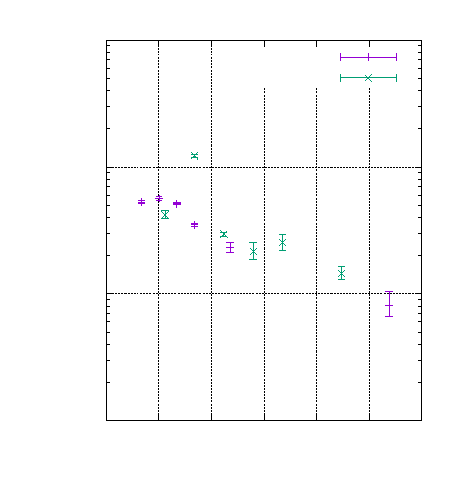
\includegraphics{cosktauconf}}%
    \gplfronttext
  \end{picture}%
\endgroup

    \caption{}
    \label{fig:cosconf}
\end{figure}

\begin{figure}
    \centering
    % GNUPLOT: LaTeX picture with Postscript
\begingroup
  \makeatletter
  \providecommand\color[2][]{%
    \GenericError{(gnuplot) \space\space\space\@spaces}{%
      Package color not loaded in conjunction with
      terminal option `colourtext'%
    }{See the gnuplot documentation for explanation.%
    }{Either use 'blacktext' in gnuplot or load the package
      color.sty in LaTeX.}%
    \renewcommand\color[2][]{}%
  }%
  \providecommand\includegraphics[2][]{%
    \GenericError{(gnuplot) \space\space\space\@spaces}{%
      Package graphicx or graphics not loaded%
    }{See the gnuplot documentation for explanation.%
    }{The gnuplot epslatex terminal needs graphicx.sty or graphics.sty.}%
    \renewcommand\includegraphics[2][]{}%
  }%
  \providecommand\rotatebox[2]{#2}%
  \@ifundefined{ifGPcolor}{%
    \newif\ifGPcolor
    \GPcolortrue
  }{}%
  \@ifundefined{ifGPblacktext}{%
    \newif\ifGPblacktext
    \GPblacktexttrue
  }{}%
  % define a \g@addto@macro without @ in the name:
  \let\gplgaddtomacro\g@addto@macro
  % define empty templates for all commands taking text:
  \gdef\gplbacktext{}%
  \gdef\gplfronttext{}%
  \makeatother
  \ifGPblacktext
    % no textcolor at all
    \def\colorrgb#1{}%
    \def\colorgray#1{}%
  \else
    % gray or color?
    \ifGPcolor
      \def\colorrgb#1{\color[rgb]{#1}}%
      \def\colorgray#1{\color[gray]{#1}}%
      \expandafter\def\csname LTw\endcsname{\color{white}}%
      \expandafter\def\csname LTb\endcsname{\color{black}}%
      \expandafter\def\csname LTa\endcsname{\color{black}}%
      \expandafter\def\csname LT0\endcsname{\color[rgb]{1,0,0}}%
      \expandafter\def\csname LT1\endcsname{\color[rgb]{0,1,0}}%
      \expandafter\def\csname LT2\endcsname{\color[rgb]{0,0,1}}%
      \expandafter\def\csname LT3\endcsname{\color[rgb]{1,0,1}}%
      \expandafter\def\csname LT4\endcsname{\color[rgb]{0,1,1}}%
      \expandafter\def\csname LT5\endcsname{\color[rgb]{1,1,0}}%
      \expandafter\def\csname LT6\endcsname{\color[rgb]{0,0,0}}%
      \expandafter\def\csname LT7\endcsname{\color[rgb]{1,0.3,0}}%
      \expandafter\def\csname LT8\endcsname{\color[rgb]{0.5,0.5,0.5}}%
    \else
      % gray
      \def\colorrgb#1{\color{black}}%
      \def\colorgray#1{\color[gray]{#1}}%
      \expandafter\def\csname LTw\endcsname{\color{white}}%
      \expandafter\def\csname LTb\endcsname{\color{black}}%
      \expandafter\def\csname LTa\endcsname{\color{black}}%
      \expandafter\def\csname LT0\endcsname{\color{black}}%
      \expandafter\def\csname LT1\endcsname{\color{black}}%
      \expandafter\def\csname LT2\endcsname{\color{black}}%
      \expandafter\def\csname LT3\endcsname{\color{black}}%
      \expandafter\def\csname LT4\endcsname{\color{black}}%
      \expandafter\def\csname LT5\endcsname{\color{black}}%
      \expandafter\def\csname LT6\endcsname{\color{black}}%
      \expandafter\def\csname LT7\endcsname{\color{black}}%
      \expandafter\def\csname LT8\endcsname{\color{black}}%
    \fi
  \fi
  \setlength{\unitlength}{0.0500bp}%
  \begin{picture}(4080.00,3400.00)%
    \gplgaddtomacro\gplbacktext{%
      \csname LTb\endcsname%
      \put(740,1058){\makebox(0,0)[r]{\strut{}1}}%
      \csname LTb\endcsname%
      \put(740,2109){\makebox(0,0)[r]{\strut{}10}}%
      \csname LTb\endcsname%
      \put(740,3159){\makebox(0,0)[r]{\strut{}100}}%
      \csname LTb\endcsname%
      \put(860,440){\makebox(0,0){\strut{}0}}%
      \csname LTb\endcsname%
      \put(1337,440){\makebox(0,0){\strut{}0.2}}%
      \csname LTb\endcsname%
      \put(1813,440){\makebox(0,0){\strut{}0.4}}%
      \csname LTb\endcsname%
      \put(2290,440){\makebox(0,0){\strut{}0.6}}%
      \csname LTb\endcsname%
      \put(2766,440){\makebox(0,0){\strut{}0.8}}%
      \csname LTb\endcsname%
      \put(3243,440){\makebox(0,0){\strut{}1}}%
      \csname LTb\endcsname%
      \put(3719,440){\makebox(0,0){\strut{}1.2}}%
      \put(160,1899){\rotatebox{-270}{\makebox(0,0){\strut{}$\tau$ /[s]}}}%
      \put(2289,140){\makebox(0,0){\strut{}$k$ /[$\micro$m$^{-1}$]}}%
    }%
    \gplgaddtomacro\gplfronttext{%
      \csname LTb\endcsname%
      \put(3128,2935){\makebox(0,0)[r]{\strut{}Fri sträng nr. 1}}%
      \csname LTb\endcsname%
      \put(3128,2735){\makebox(0,0)[r]{\strut{}Fri sträng nr. 2}}%
    }%
    \gplbacktext
    \put(0,0){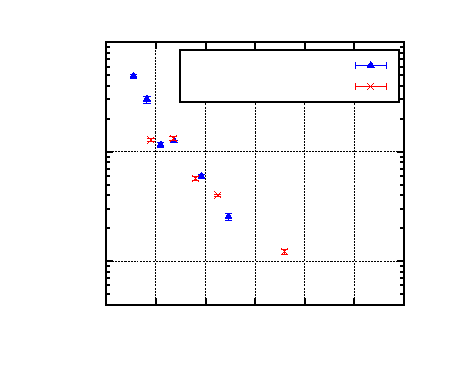
\includegraphics{cosktaunonconf}}%
    \gplfronttext
  \end{picture}%
\endgroup

    \caption{}
    \label{fig:cosnonconf}
\end{figure}

\section{Egenmoder -- }


Metoden för sönderläggning av strängens rörelse i egenmoder beskrivs i avsnitt \ref{sec:kovmatris} som en diagonalisering av kovariansmatrisen, där kovariansmatrisen $C$ i detta fallet byggs upp av avståndskomponenter till strängen. %Hädanefter betecknas därför det transversella avståndet till strängen relativt sitt jämviktsläge $A_s(t)$ där $s$ är en diskret båglängdsparameter längs med strängen.
Diagonalisering av denna kovariansmatris med hjälp av spektralsatsen leder effektivt till ett basbyte från en bas bestående av det transversella avståndet i varje $s$ längs strängen, till en bas bestående av egenmoderna för strängen. %Egenvärdena till kovariansmatrisen ger ett mått på hur mycket av strängens rörelse som byggs upp av motsvarande egenmod. 
Genom att projicera strängens rörelse på ett fåtal av de egenmoder med störst egenvärde förenklas analysen\cite{Shlens_PCA2014}; karakteristiska egenskaper för varje egenmod kan undersökas separat. Hädanefter betecknas därför det transversella avståndet till strängen relativt sitt jämviktsläge $A_s(t)$ där $s$ är en \emph{diskret} båglängdsparameter längs med strängen.

Kovariansmatrisen bildad av $A_s(t)$ kan bildas enligt \eqref{eq:kovmatris} som 
\begin{equation}
\label{eq:C}
    C_{ij} = \COV{A_s(t)}{A_{s'}(t)}_t.
\end{equation}
Egenvektorerna till $C$, hädanefter egenmoderna, betecknas $\mathbf{B}_i$ och strängrörelsen kan representeras som
\begin{equation}
    A_s(t) = \sum_i^n \alpha_{si}(t)B_i,
\end{equation}
$\hat{\mathbf{A}}_s$ är en enhetsvektor längs komponent $s$ och 
\begin{equation}
    \alpha_{si}(t) = A_s(t)\mathbf{B}_i\cdot\hat{\mathbf{A}}_s.
\end{equation}
Projektionen av strängrörelsen på varje egenmod som funktion av tiden beskrivs av
\begin{equation}
    b_i(t) = \sum_s^n \alpha_{si}(t).
\end{equation}

Autokorrelationsfunktionen för varje komponent $b_i(t)$ innehåller information om strängrörelsens tidsutveckling, genom att endast betrakta de komponenter med ''tillräckligt'' stora egenvärden förenklas analysen och relaxationstider för de mest dominanta egenmoderna tas fram från 
\begin{equation}
    \ev{b_i(t)b_i(t+\Delta t)}.
\end{equation}
Antalet egenvärden som är tillräckligt att studera beror på hur väl man vill beskriva rörelsen. Det finns flera modeller för att bestämma hur många egenvärden som behövs, men enligt \cite{Cangelosi2007} så förutspår dessa inte alltid entydiga svar. 

\subsection{Resultat -- Signifikanta egenmoder}

Egenvärdena till kovariansmatrisen bildad från de stokastiska processerna $A_s(t)$ visar en tydlig spridning, där $\lambda_\text{max}/\lambda_\text{min}\geq 10^{16}$ och är oberoende av strängtyp vilket ses i figur \ref{fig:kovegenvarde}. Den stora skillnaden i varians visar att strängrörelsen till en god approximation kan beskrivas i ett fåtal egenmoder snarare än separata avstånd i varje punkt längs strängen. 

%Antalet egenvärde \sim polynomgrad


\begin{figure}
    \centering
    % GNUPLOT: LaTeX picture with Postscript
\begingroup
  \makeatletter
  \providecommand\color[2][]{%
    \GenericError{(gnuplot) \space\space\space\@spaces}{%
      Package color not loaded in conjunction with
      terminal option `colourtext'%
    }{See the gnuplot documentation for explanation.%
    }{Either use 'blacktext' in gnuplot or load the package
      color.sty in LaTeX.}%
    \renewcommand\color[2][]{}%
  }%
  \providecommand\includegraphics[2][]{%
    \GenericError{(gnuplot) \space\space\space\@spaces}{%
      Package graphicx or graphics not loaded%
    }{See the gnuplot documentation for explanation.%
    }{The gnuplot epslatex terminal needs graphicx.sty or graphics.sty.}%
    \renewcommand\includegraphics[2][]{}%
  }%
  \providecommand\rotatebox[2]{#2}%
  \@ifundefined{ifGPcolor}{%
    \newif\ifGPcolor
    \GPcolortrue
  }{}%
  \@ifundefined{ifGPblacktext}{%
    \newif\ifGPblacktext
    \GPblacktexttrue
  }{}%
  % define a \g@addto@macro without @ in the name:
  \let\gplgaddtomacro\g@addto@macro
  % define empty templates for all commands taking text:
  \gdef\gplbacktext{}%
  \gdef\gplfronttext{}%
  \makeatother
  \ifGPblacktext
    % no textcolor at all
    \def\colorrgb#1{}%
    \def\colorgray#1{}%
  \else
    % gray or color?
    \ifGPcolor
      \def\colorrgb#1{\color[rgb]{#1}}%
      \def\colorgray#1{\color[gray]{#1}}%
      \expandafter\def\csname LTw\endcsname{\color{white}}%
      \expandafter\def\csname LTb\endcsname{\color{black}}%
      \expandafter\def\csname LTa\endcsname{\color{black}}%
      \expandafter\def\csname LT0\endcsname{\color[rgb]{1,0,0}}%
      \expandafter\def\csname LT1\endcsname{\color[rgb]{0,1,0}}%
      \expandafter\def\csname LT2\endcsname{\color[rgb]{0,0,1}}%
      \expandafter\def\csname LT3\endcsname{\color[rgb]{1,0,1}}%
      \expandafter\def\csname LT4\endcsname{\color[rgb]{0,1,1}}%
      \expandafter\def\csname LT5\endcsname{\color[rgb]{1,1,0}}%
      \expandafter\def\csname LT6\endcsname{\color[rgb]{0,0,0}}%
      \expandafter\def\csname LT7\endcsname{\color[rgb]{1,0.3,0}}%
      \expandafter\def\csname LT8\endcsname{\color[rgb]{0.5,0.5,0.5}}%
    \else
      % gray
      \def\colorrgb#1{\color{black}}%
      \def\colorgray#1{\color[gray]{#1}}%
      \expandafter\def\csname LTw\endcsname{\color{white}}%
      \expandafter\def\csname LTb\endcsname{\color{black}}%
      \expandafter\def\csname LTa\endcsname{\color{black}}%
      \expandafter\def\csname LT0\endcsname{\color{black}}%
      \expandafter\def\csname LT1\endcsname{\color{black}}%
      \expandafter\def\csname LT2\endcsname{\color{black}}%
      \expandafter\def\csname LT3\endcsname{\color{black}}%
      \expandafter\def\csname LT4\endcsname{\color{black}}%
      \expandafter\def\csname LT5\endcsname{\color{black}}%
      \expandafter\def\csname LT6\endcsname{\color{black}}%
      \expandafter\def\csname LT7\endcsname{\color{black}}%
      \expandafter\def\csname LT8\endcsname{\color{black}}%
    \fi
  \fi
    \setlength{\unitlength}{0.0500bp}%
    \ifx\gptboxheight\undefined%
      \newlength{\gptboxheight}%
      \newlength{\gptboxwidth}%
      \newsavebox{\gptboxtext}%
    \fi%
    \setlength{\fboxrule}{0.5pt}%
    \setlength{\fboxsep}{1pt}%
\begin{picture}(6802.00,4534.00)%
    \gplgaddtomacro\gplbacktext{%
      \csname LTb\endcsname%
      \put(980,814){\makebox(0,0)[r]{\strut{}$10^{-29}$}}%
      \csname LTb\endcsname%
      \put(980,1510){\makebox(0,0)[r]{\strut{}$10^{-25}$}}%
      \csname LTb\endcsname%
      \put(980,2206){\makebox(0,0)[r]{\strut{}$10^{-21}$}}%
      \csname LTb\endcsname%
      \put(980,2901){\makebox(0,0)[r]{\strut{}$10^{-17}$}}%
      \csname LTb\endcsname%
      \put(980,3597){\makebox(0,0)[r]{\strut{}$10^{-13}$}}%
      \csname LTb\endcsname%
      \put(980,4293){\makebox(0,0)[r]{\strut{}$10^{-9}$}}%
      \csname LTb\endcsname%
      \put(1314,440){\makebox(0,0){\strut{}$20$}}%
      \csname LTb\endcsname%
      \put(2168,440){\makebox(0,0){\strut{}$40$}}%
      \csname LTb\endcsname%
      \put(3023,440){\makebox(0,0){\strut{}$60$}}%
      \csname LTb\endcsname%
      \put(3877,440){\makebox(0,0){\strut{}$80$}}%
      \csname LTb\endcsname%
      \put(4732,440){\makebox(0,0){\strut{}$100$}}%
      \csname LTb\endcsname%
      \put(5586,440){\makebox(0,0){\strut{}$120$}}%
      \csname LTb\endcsname%
      \put(6441,440){\makebox(0,0){\strut{}$140$}}%
    }%
    \gplgaddtomacro\gplfronttext{%
      \csname LTb\endcsname%
      \put(160,2466){\rotatebox{-270}{\makebox(0,0){\strut{}var[B$_i$]/[m$^2$]}}}%
      \put(3770,140){\makebox(0,0){\strut{}$\lambda_k$}}%
      \csname LTb\endcsname%
      \put(2480,4130){\makebox(0,0)[r]{\strut{}confined}}%
      \csname LTb\endcsname%
      \put(2480,3930){\makebox(0,0)[r]{\strut{}confined}}%
      \csname LTb\endcsname%
      \put(2480,3730){\makebox(0,0)[r]{\strut{}non-confined}}%
      \csname LTb\endcsname%
      \put(2480,3530){\makebox(0,0)[r]{\strut{}non-confined}}%
    }%
    \gplbacktext
    \put(0,0){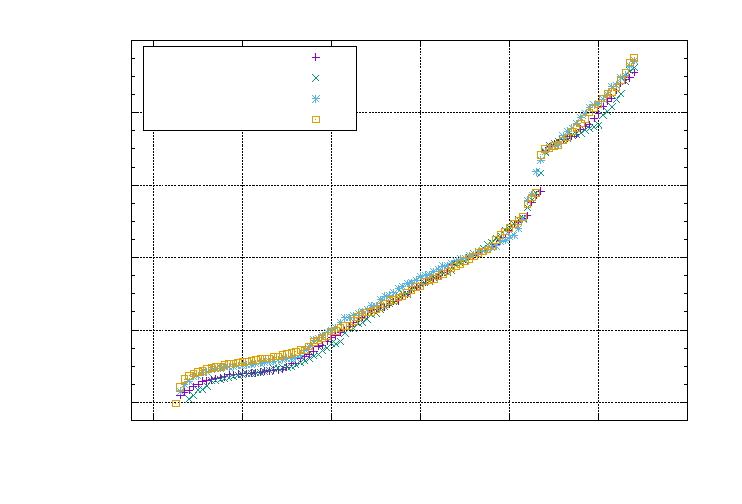
\includegraphics{kovegenv}}%
    \gplfronttext
  \end{picture}%
\endgroup

    \caption{Egenvärden till kovariansmatrisen från \eqref{eq:C} för fyra olika strängar. Det största egenvärdent ses vara åtminstone $10^{16}$ storlekar större än det minsta, vilket påvisar en signifikant skillnad i bidrag till rörelsen från vardera egenmod.}
    \label{fig:kovegenvarde}
\end{figure}

\begin{figure}
    \centering
    % GNUPLOT: LaTeX picture with Postscript
\begingroup
  \makeatletter
  \providecommand\color[2][]{%
    \GenericError{(gnuplot) \space\space\space\@spaces}{%
      Package color not loaded in conjunction with
      terminal option `colourtext'%
    }{See the gnuplot documentation for explanation.%
    }{Either use 'blacktext' in gnuplot or load the package
      color.sty in LaTeX.}%
    \renewcommand\color[2][]{}%
  }%
  \providecommand\includegraphics[2][]{%
    \GenericError{(gnuplot) \space\space\space\@spaces}{%
      Package graphicx or graphics not loaded%
    }{See the gnuplot documentation for explanation.%
    }{The gnuplot epslatex terminal needs graphicx.sty or graphics.sty.}%
    \renewcommand\includegraphics[2][]{}%
  }%
  \providecommand\rotatebox[2]{#2}%
  \@ifundefined{ifGPcolor}{%
    \newif\ifGPcolor
    \GPcolortrue
  }{}%
  \@ifundefined{ifGPblacktext}{%
    \newif\ifGPblacktext
    \GPblacktexttrue
  }{}%
  % define a \g@addto@macro without @ in the name:
  \let\gplgaddtomacro\g@addto@macro
  % define empty templates for all commands taking text:
  \gdef\gplbacktext{}%
  \gdef\gplfronttext{}%
  \makeatother
  \ifGPblacktext
    % no textcolor at all
    \def\colorrgb#1{}%
    \def\colorgray#1{}%
  \else
    % gray or color?
    \ifGPcolor
      \def\colorrgb#1{\color[rgb]{#1}}%
      \def\colorgray#1{\color[gray]{#1}}%
      \expandafter\def\csname LTw\endcsname{\color{white}}%
      \expandafter\def\csname LTb\endcsname{\color{black}}%
      \expandafter\def\csname LTa\endcsname{\color{black}}%
      \expandafter\def\csname LT0\endcsname{\color[rgb]{1,0,0}}%
      \expandafter\def\csname LT1\endcsname{\color[rgb]{0,1,0}}%
      \expandafter\def\csname LT2\endcsname{\color[rgb]{0,0,1}}%
      \expandafter\def\csname LT3\endcsname{\color[rgb]{1,0,1}}%
      \expandafter\def\csname LT4\endcsname{\color[rgb]{0,1,1}}%
      \expandafter\def\csname LT5\endcsname{\color[rgb]{1,1,0}}%
      \expandafter\def\csname LT6\endcsname{\color[rgb]{0,0,0}}%
      \expandafter\def\csname LT7\endcsname{\color[rgb]{1,0.3,0}}%
      \expandafter\def\csname LT8\endcsname{\color[rgb]{0.5,0.5,0.5}}%
    \else
      % gray
      \def\colorrgb#1{\color{black}}%
      \def\colorgray#1{\color[gray]{#1}}%
      \expandafter\def\csname LTw\endcsname{\color{white}}%
      \expandafter\def\csname LTb\endcsname{\color{black}}%
      \expandafter\def\csname LTa\endcsname{\color{black}}%
      \expandafter\def\csname LT0\endcsname{\color{black}}%
      \expandafter\def\csname LT1\endcsname{\color{black}}%
      \expandafter\def\csname LT2\endcsname{\color{black}}%
      \expandafter\def\csname LT3\endcsname{\color{black}}%
      \expandafter\def\csname LT4\endcsname{\color{black}}%
      \expandafter\def\csname LT5\endcsname{\color{black}}%
      \expandafter\def\csname LT6\endcsname{\color{black}}%
      \expandafter\def\csname LT7\endcsname{\color{black}}%
      \expandafter\def\csname LT8\endcsname{\color{black}}%
    \fi
  \fi
    \setlength{\unitlength}{0.0500bp}%
    \ifx\gptboxheight\undefined%
      \newlength{\gptboxheight}%
      \newlength{\gptboxwidth}%
      \newsavebox{\gptboxtext}%
    \fi%
    \setlength{\fboxrule}{0.5pt}%
    \setlength{\fboxsep}{1pt}%
\begin{picture}(6802.00,3968.00)%
    \gplgaddtomacro\gplbacktext{%
      \csname LTb\endcsname%
      \put(980,640){\makebox(0,0)[r]{\strut{}$10^{-13}$}}%
      \csname LTb\endcsname%
      \put(980,1726){\makebox(0,0)[r]{\strut{}$10^{-12}$}}%
      \csname LTb\endcsname%
      \put(980,2812){\makebox(0,0)[r]{\strut{}$10^{-11}$}}%
      \csname LTb\endcsname%
      \put(1100,440){\makebox(0,0){\strut{}$0$}}%
      \csname LTb\endcsname%
      \put(2435,440){\makebox(0,0){\strut{}$0.5$}}%
      \csname LTb\endcsname%
      \put(3771,440){\makebox(0,0){\strut{}$1$}}%
      \csname LTb\endcsname%
      \put(5106,440){\makebox(0,0){\strut{}$1.5$}}%
      \csname LTb\endcsname%
      \put(6441,440){\makebox(0,0){\strut{}$2$}}%
    }%
    \gplgaddtomacro\gplfronttext{%
      \csname LTb\endcsname%
      \put(160,2183){\rotatebox{-270}{\makebox(0,0){\strut{}$\ev{B_{i}(t)B_{i}(t+\Delta t)}$}}}%
      \put(3770,140){\makebox(0,0){\strut{}$\Delta t$/[s]}}%
    }%
    \gplbacktext
    \put(0,0){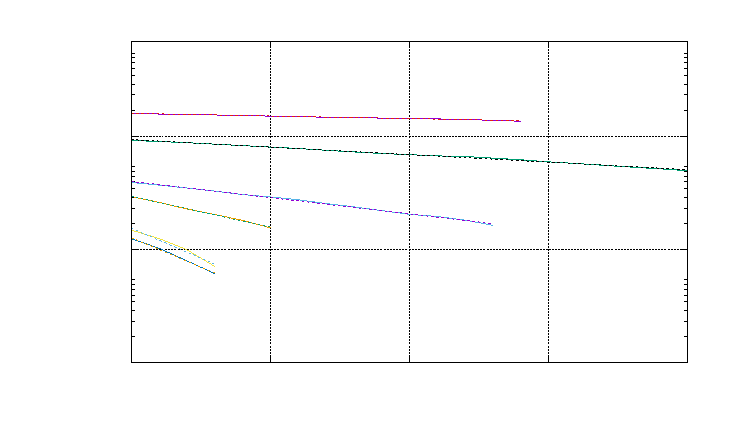
\includegraphics{korrfil3}}%
    \gplfronttext
  \end{picture}%
\endgroup

    \caption{\textcolor{red}{\Large Lägg till markörer vid varje data punkt så att alla ser mot vad anpassningarna har gjorts.}}
    \label{fig:korrelation}
\end{figure}

\begin{figure}
    \centering
    % GNUPLOT: LaTeX picture with Postscript
\begingroup
  \makeatletter
  \providecommand\color[2][]{%
    \GenericError{(gnuplot) \space\space\space\@spaces}{%
      Package color not loaded in conjunction with
      terminal option `colourtext'%
    }{See the gnuplot documentation for explanation.%
    }{Either use 'blacktext' in gnuplot or load the package
      color.sty in LaTeX.}%
    \renewcommand\color[2][]{}%
  }%
  \providecommand\includegraphics[2][]{%
    \GenericError{(gnuplot) \space\space\space\@spaces}{%
      Package graphicx or graphics not loaded%
    }{See the gnuplot documentation for explanation.%
    }{The gnuplot epslatex terminal needs graphicx.sty or graphics.sty.}%
    \renewcommand\includegraphics[2][]{}%
  }%
  \providecommand\rotatebox[2]{#2}%
  \@ifundefined{ifGPcolor}{%
    \newif\ifGPcolor
    \GPcolortrue
  }{}%
  \@ifundefined{ifGPblacktext}{%
    \newif\ifGPblacktext
    \GPblacktexttrue
  }{}%
  % define a \g@addto@macro without @ in the name:
  \let\gplgaddtomacro\g@addto@macro
  % define empty templates for all commands taking text:
  \gdef\gplbacktext{}%
  \gdef\gplfronttext{}%
  \makeatother
  \ifGPblacktext
    % no textcolor at all
    \def\colorrgb#1{}%
    \def\colorgray#1{}%
  \else
    % gray or color?
    \ifGPcolor
      \def\colorrgb#1{\color[rgb]{#1}}%
      \def\colorgray#1{\color[gray]{#1}}%
      \expandafter\def\csname LTw\endcsname{\color{white}}%
      \expandafter\def\csname LTb\endcsname{\color{black}}%
      \expandafter\def\csname LTa\endcsname{\color{black}}%
      \expandafter\def\csname LT0\endcsname{\color[rgb]{1,0,0}}%
      \expandafter\def\csname LT1\endcsname{\color[rgb]{0,1,0}}%
      \expandafter\def\csname LT2\endcsname{\color[rgb]{0,0,1}}%
      \expandafter\def\csname LT3\endcsname{\color[rgb]{1,0,1}}%
      \expandafter\def\csname LT4\endcsname{\color[rgb]{0,1,1}}%
      \expandafter\def\csname LT5\endcsname{\color[rgb]{1,1,0}}%
      \expandafter\def\csname LT6\endcsname{\color[rgb]{0,0,0}}%
      \expandafter\def\csname LT7\endcsname{\color[rgb]{1,0.3,0}}%
      \expandafter\def\csname LT8\endcsname{\color[rgb]{0.5,0.5,0.5}}%
    \else
      % gray
      \def\colorrgb#1{\color{black}}%
      \def\colorgray#1{\color[gray]{#1}}%
      \expandafter\def\csname LTw\endcsname{\color{white}}%
      \expandafter\def\csname LTb\endcsname{\color{black}}%
      \expandafter\def\csname LTa\endcsname{\color{black}}%
      \expandafter\def\csname LT0\endcsname{\color{black}}%
      \expandafter\def\csname LT1\endcsname{\color{black}}%
      \expandafter\def\csname LT2\endcsname{\color{black}}%
      \expandafter\def\csname LT3\endcsname{\color{black}}%
      \expandafter\def\csname LT4\endcsname{\color{black}}%
      \expandafter\def\csname LT5\endcsname{\color{black}}%
      \expandafter\def\csname LT6\endcsname{\color{black}}%
      \expandafter\def\csname LT7\endcsname{\color{black}}%
      \expandafter\def\csname LT8\endcsname{\color{black}}%
    \fi
  \fi
    \setlength{\unitlength}{0.0500bp}%
    \ifx\gptboxheight\undefined%
      \newlength{\gptboxheight}%
      \newlength{\gptboxwidth}%
      \newsavebox{\gptboxtext}%
    \fi%
    \setlength{\fboxrule}{0.5pt}%
    \setlength{\fboxsep}{1pt}%
\begin{picture}(6802.00,3968.00)%
    \gplgaddtomacro\gplbacktext{%
      \csname LTb\endcsname%
      \put(980,640){\makebox(0,0)[r]{\strut{}$-0,15$}}%
      \csname LTb\endcsname%
      \put(980,1026){\makebox(0,0)[r]{\strut{}$-0,1$}}%
      \csname LTb\endcsname%
      \put(980,1412){\makebox(0,0)[r]{\strut{}$-0,05$}}%
      \csname LTb\endcsname%
      \put(980,1798){\makebox(0,0)[r]{\strut{}$0$}}%
      \csname LTb\endcsname%
      \put(980,2184){\makebox(0,0)[r]{\strut{}$0,05$}}%
      \csname LTb\endcsname%
      \put(980,2569){\makebox(0,0)[r]{\strut{}$0,1$}}%
      \csname LTb\endcsname%
      \put(980,2955){\makebox(0,0)[r]{\strut{}$0,15$}}%
      \csname LTb\endcsname%
      \put(980,3341){\makebox(0,0)[r]{\strut{}$0,2$}}%
      \csname LTb\endcsname%
      \put(980,3727){\makebox(0,0)[r]{\strut{}$0,25$}}%
      \csname LTb\endcsname%
      \put(1100,440){\makebox(0,0){\strut{}$0$}}%
      \csname LTb\endcsname%
      \put(1863,440){\makebox(0,0){\strut{}$5$}}%
      \csname LTb\endcsname%
      \put(2626,440){\makebox(0,0){\strut{}$10$}}%
      \csname LTb\endcsname%
      \put(3389,440){\makebox(0,0){\strut{}$15$}}%
      \csname LTb\endcsname%
      \put(4152,440){\makebox(0,0){\strut{}$20$}}%
      \csname LTb\endcsname%
      \put(4915,440){\makebox(0,0){\strut{}$25$}}%
      \csname LTb\endcsname%
      \put(5678,440){\makebox(0,0){\strut{}$30$}}%
      \csname LTb\endcsname%
      \put(6441,440){\makebox(0,0){\strut{}$35$}}%
    }%
    \gplgaddtomacro\gplfronttext{%
      \csname LTb\endcsname%
      \put(160,2183){\rotatebox{-270}{\makebox(0,0){\strut{}$v_i(l)$}}}%
      \put(3770,140){\makebox(0,0){\strut{}$l$ /[$\micro$m]}}%
      \csname LTb\endcsname%
      \put(2776,3514){\makebox(0,0)[r]{\strut{}$\mathbf{B}_2$}}%
      \csname LTb\endcsname%
      \put(3679,3514){\makebox(0,0)[r]{\strut{}$\mathbf{B}_3$}}%
      \csname LTb\endcsname%
      \put(4582,3514){\makebox(0,0)[r]{\strut{}$\mathbf{B}_4$}}%
    }%
    \gplbacktext
    \put(0,0){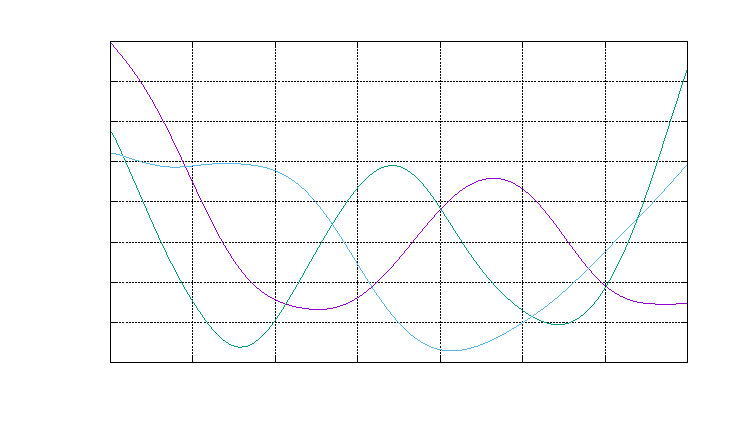
\includegraphics{moder}}%
    \gplfronttext
  \end{picture}%
\endgroup

    \caption{\textcolor{red}{\Large Ändra så att det blir streckade linjer för olika moder (svart-vit-anpassa).}}
    \label{fig:egenmoder}
\end{figure}

\begin{figure}
    \centering
    % GNUPLOT: LaTeX picture with Postscript
\begingroup
  \makeatletter
  \providecommand\color[2][]{%
    \GenericError{(gnuplot) \space\space\space\@spaces}{%
      Package color not loaded in conjunction with
      terminal option `colourtext'%
    }{See the gnuplot documentation for explanation.%
    }{Either use 'blacktext' in gnuplot or load the package
      color.sty in LaTeX.}%
    \renewcommand\color[2][]{}%
  }%
  \providecommand\includegraphics[2][]{%
    \GenericError{(gnuplot) \space\space\space\@spaces}{%
      Package graphicx or graphics not loaded%
    }{See the gnuplot documentation for explanation.%
    }{The gnuplot epslatex terminal needs graphicx.sty or graphics.sty.}%
    \renewcommand\includegraphics[2][]{}%
  }%
  \providecommand\rotatebox[2]{#2}%
  \@ifundefined{ifGPcolor}{%
    \newif\ifGPcolor
    \GPcolortrue
  }{}%
  \@ifundefined{ifGPblacktext}{%
    \newif\ifGPblacktext
    \GPblacktexttrue
  }{}%
  % define a \g@addto@macro without @ in the name:
  \let\gplgaddtomacro\g@addto@macro
  % define empty templates for all commands taking text:
  \gdef\gplbacktext{}%
  \gdef\gplfronttext{}%
  \makeatother
  \ifGPblacktext
    % no textcolor at all
    \def\colorrgb#1{}%
    \def\colorgray#1{}%
  \else
    % gray or color?
    \ifGPcolor
      \def\colorrgb#1{\color[rgb]{#1}}%
      \def\colorgray#1{\color[gray]{#1}}%
      \expandafter\def\csname LTw\endcsname{\color{white}}%
      \expandafter\def\csname LTb\endcsname{\color{black}}%
      \expandafter\def\csname LTa\endcsname{\color{black}}%
      \expandafter\def\csname LT0\endcsname{\color[rgb]{1,0,0}}%
      \expandafter\def\csname LT1\endcsname{\color[rgb]{0,1,0}}%
      \expandafter\def\csname LT2\endcsname{\color[rgb]{0,0,1}}%
      \expandafter\def\csname LT3\endcsname{\color[rgb]{1,0,1}}%
      \expandafter\def\csname LT4\endcsname{\color[rgb]{0,1,1}}%
      \expandafter\def\csname LT5\endcsname{\color[rgb]{1,1,0}}%
      \expandafter\def\csname LT6\endcsname{\color[rgb]{0,0,0}}%
      \expandafter\def\csname LT7\endcsname{\color[rgb]{1,0.3,0}}%
      \expandafter\def\csname LT8\endcsname{\color[rgb]{0.5,0.5,0.5}}%
    \else
      % gray
      \def\colorrgb#1{\color{black}}%
      \def\colorgray#1{\color[gray]{#1}}%
      \expandafter\def\csname LTw\endcsname{\color{white}}%
      \expandafter\def\csname LTb\endcsname{\color{black}}%
      \expandafter\def\csname LTa\endcsname{\color{black}}%
      \expandafter\def\csname LT0\endcsname{\color{black}}%
      \expandafter\def\csname LT1\endcsname{\color{black}}%
      \expandafter\def\csname LT2\endcsname{\color{black}}%
      \expandafter\def\csname LT3\endcsname{\color{black}}%
      \expandafter\def\csname LT4\endcsname{\color{black}}%
      \expandafter\def\csname LT5\endcsname{\color{black}}%
      \expandafter\def\csname LT6\endcsname{\color{black}}%
      \expandafter\def\csname LT7\endcsname{\color{black}}%
      \expandafter\def\csname LT8\endcsname{\color{black}}%
    \fi
  \fi
    \setlength{\unitlength}{0.0500bp}%
    \ifx\gptboxheight\undefined%
      \newlength{\gptboxheight}%
      \newlength{\gptboxwidth}%
      \newsavebox{\gptboxtext}%
    \fi%
    \setlength{\fboxrule}{0.5pt}%
    \setlength{\fboxsep}{1pt}%
\begin{picture}(6802.00,3968.00)%
    \gplgaddtomacro\gplbacktext{%
      \csname LTb\endcsname%
      \put(780,640){\makebox(0,0)[r]{\strut{}$-0.15$}}%
      \csname LTb\endcsname%
      \put(780,1155){\makebox(0,0)[r]{\strut{}$-0.1$}}%
      \csname LTb\endcsname%
      \put(780,1669){\makebox(0,0)[r]{\strut{}$-0.05$}}%
      \csname LTb\endcsname%
      \put(780,2184){\makebox(0,0)[r]{\strut{}$0$}}%
      \csname LTb\endcsname%
      \put(780,2698){\makebox(0,0)[r]{\strut{}$0.05$}}%
      \csname LTb\endcsname%
      \put(780,3212){\makebox(0,0)[r]{\strut{}$0.1$}}%
      \csname LTb\endcsname%
      \put(780,3727){\makebox(0,0)[r]{\strut{}$0.15$}}%
      \csname LTb\endcsname%
      \put(900,440){\makebox(0,0){\strut{}$0$}}%
      \csname LTb\endcsname%
      \put(1692,440){\makebox(0,0){\strut{}$5$}}%
      \csname LTb\endcsname%
      \put(2483,440){\makebox(0,0){\strut{}$10$}}%
      \csname LTb\endcsname%
      \put(3275,440){\makebox(0,0){\strut{}$15$}}%
      \csname LTb\endcsname%
      \put(4066,440){\makebox(0,0){\strut{}$20$}}%
      \csname LTb\endcsname%
      \put(4858,440){\makebox(0,0){\strut{}$25$}}%
      \csname LTb\endcsname%
      \put(5649,440){\makebox(0,0){\strut{}$30$}}%
      \csname LTb\endcsname%
      \put(6441,440){\makebox(0,0){\strut{}$35$}}%
    }%
    \gplgaddtomacro\gplfronttext{%
      \csname LTb\endcsname%
      \put(3670,140){\makebox(0,0){\strut{}$l$/[$\micro$m]}}%
    }%
    \gplbacktext
    \put(0,0){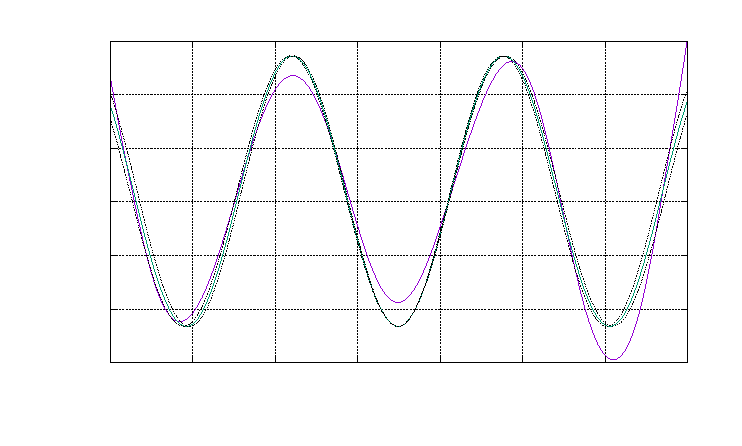
\includegraphics{modkorrektion}}%
    \gplfronttext
  \end{picture}%
\endgroup

    \caption{\textcolor{red}{\Large Ändra så att det blir streckade linjer för anpassnigarna.}
}
    \label{fig:modkorrektion}
\end{figure}


\begin{figure}\centerline{
\subfigure[][]{
% GNUPLOT: LaTeX picture with Postscript
\begingroup
  \makeatletter
  \providecommand\color[2][]{%
    \GenericError{(gnuplot) \space\space\space\@spaces}{%
      Package color not loaded in conjunction with
      terminal option `colourtext'%
    }{See the gnuplot documentation for explanation.%
    }{Either use 'blacktext' in gnuplot or load the package
      color.sty in LaTeX.}%
    \renewcommand\color[2][]{}%
  }%
  \providecommand\includegraphics[2][]{%
    \GenericError{(gnuplot) \space\space\space\@spaces}{%
      Package graphicx or graphics not loaded%
    }{See the gnuplot documentation for explanation.%
    }{The gnuplot epslatex terminal needs graphicx.sty or graphics.sty.}%
    \renewcommand\includegraphics[2][]{}%
  }%
  \providecommand\rotatebox[2]{#2}%
  \@ifundefined{ifGPcolor}{%
    \newif\ifGPcolor
    \GPcolortrue
  }{}%
  \@ifundefined{ifGPblacktext}{%
    \newif\ifGPblacktext
    \GPblacktexttrue
  }{}%
  % define a \g@addto@macro without @ in the name:
  \let\gplgaddtomacro\g@addto@macro
  % define empty templates for all commands taking text:
  \gdef\gplbacktext{}%
  \gdef\gplfronttext{}%
  \makeatother
  \ifGPblacktext
    % no textcolor at all
    \def\colorrgb#1{}%
    \def\colorgray#1{}%
  \else
    % gray or color?
    \ifGPcolor
      \def\colorrgb#1{\color[rgb]{#1}}%
      \def\colorgray#1{\color[gray]{#1}}%
      \expandafter\def\csname LTw\endcsname{\color{white}}%
      \expandafter\def\csname LTb\endcsname{\color{black}}%
      \expandafter\def\csname LTa\endcsname{\color{black}}%
      \expandafter\def\csname LT0\endcsname{\color[rgb]{1,0,0}}%
      \expandafter\def\csname LT1\endcsname{\color[rgb]{0,1,0}}%
      \expandafter\def\csname LT2\endcsname{\color[rgb]{0,0,1}}%
      \expandafter\def\csname LT3\endcsname{\color[rgb]{1,0,1}}%
      \expandafter\def\csname LT4\endcsname{\color[rgb]{0,1,1}}%
      \expandafter\def\csname LT5\endcsname{\color[rgb]{1,1,0}}%
      \expandafter\def\csname LT6\endcsname{\color[rgb]{0,0,0}}%
      \expandafter\def\csname LT7\endcsname{\color[rgb]{1,0.3,0}}%
      \expandafter\def\csname LT8\endcsname{\color[rgb]{0.5,0.5,0.5}}%
    \else
      % gray
      \def\colorrgb#1{\color{black}}%
      \def\colorgray#1{\color[gray]{#1}}%
      \expandafter\def\csname LTw\endcsname{\color{white}}%
      \expandafter\def\csname LTb\endcsname{\color{black}}%
      \expandafter\def\csname LTa\endcsname{\color{black}}%
      \expandafter\def\csname LT0\endcsname{\color{black}}%
      \expandafter\def\csname LT1\endcsname{\color{black}}%
      \expandafter\def\csname LT2\endcsname{\color{black}}%
      \expandafter\def\csname LT3\endcsname{\color{black}}%
      \expandafter\def\csname LT4\endcsname{\color{black}}%
      \expandafter\def\csname LT5\endcsname{\color{black}}%
      \expandafter\def\csname LT6\endcsname{\color{black}}%
      \expandafter\def\csname LT7\endcsname{\color{black}}%
      \expandafter\def\csname LT8\endcsname{\color{black}}%
    \fi
  \fi
    \setlength{\unitlength}{0.0500bp}%
    \ifx\gptboxheight\undefined%
      \newlength{\gptboxheight}%
      \newlength{\gptboxwidth}%
      \newsavebox{\gptboxtext}%
    \fi%
    \setlength{\fboxrule}{0.5pt}%
    \setlength{\fboxsep}{1pt}%
\begin{picture}(4250.00,4534.00)%
    \gplgaddtomacro\gplbacktext{%
      \csname LTb\endcsname%
      \put(740,640){\makebox(0,0)[r]{\strut{}0.1}}%
      \csname LTb\endcsname%
      \put(740,2467){\makebox(0,0)[r]{\strut{}1}}%
      \csname LTb\endcsname%
      \put(740,4293){\makebox(0,0)[r]{\strut{}10}}%
      \csname LTb\endcsname%
      \put(860,440){\makebox(0,0){\strut{}0}}%
      \csname LTb\endcsname%
      \put(1466,440){\makebox(0,0){\strut{}0.2}}%
      \csname LTb\endcsname%
      \put(2072,440){\makebox(0,0){\strut{}0.4}}%
      \csname LTb\endcsname%
      \put(2677,440){\makebox(0,0){\strut{}0.6}}%
      \csname LTb\endcsname%
      \put(3283,440){\makebox(0,0){\strut{}0.8}}%
      \csname LTb\endcsname%
      \put(3889,440){\makebox(0,0){\strut{}1}}%
    }%
    \gplgaddtomacro\gplfronttext{%
      \csname LTb\endcsname%
      \put(160,2466){\rotatebox{-270}{\makebox(0,0){\strut{}$\tau$/[s]}}}%
      \put(2374,140){\makebox(0,0){\strut{}$k$/[$\micro$m$^{-1}$]}}%
      \csname LTb\endcsname%
      \put(2986,4130){\makebox(0,0)[r]{\strut{}confined}}%
      \csname LTb\endcsname%
      \put(2986,3930){\makebox(0,0)[r]{\strut{}confined}}%
    }%
    \gplbacktext
    \put(0,0){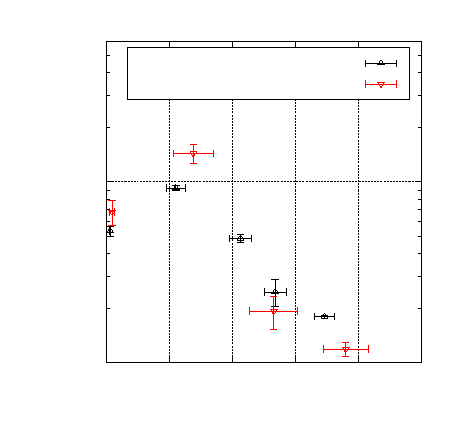
\includegraphics{ktauconf}}%
    \gplfronttext
  \end{picture}%
\endgroup

}
\subfigure[][]{
% GNUPLOT: LaTeX picture with Postscript
\begingroup
  \makeatletter
  \providecommand\color[2][]{%
    \GenericError{(gnuplot) \space\space\space\@spaces}{%
      Package color not loaded in conjunction with
      terminal option `colourtext'%
    }{See the gnuplot documentation for explanation.%
    }{Either use 'blacktext' in gnuplot or load the package
      color.sty in LaTeX.}%
    \renewcommand\color[2][]{}%
  }%
  \providecommand\includegraphics[2][]{%
    \GenericError{(gnuplot) \space\space\space\@spaces}{%
      Package graphicx or graphics not loaded%
    }{See the gnuplot documentation for explanation.%
    }{The gnuplot epslatex terminal needs graphicx.sty or graphics.sty.}%
    \renewcommand\includegraphics[2][]{}%
  }%
  \providecommand\rotatebox[2]{#2}%
  \@ifundefined{ifGPcolor}{%
    \newif\ifGPcolor
    \GPcolortrue
  }{}%
  \@ifundefined{ifGPblacktext}{%
    \newif\ifGPblacktext
    \GPblacktexttrue
  }{}%
  % define a \g@addto@macro without @ in the name:
  \let\gplgaddtomacro\g@addto@macro
  % define empty templates for all commands taking text:
  \gdef\gplbacktext{}%
  \gdef\gplfronttext{}%
  \makeatother
  \ifGPblacktext
    % no textcolor at all
    \def\colorrgb#1{}%
    \def\colorgray#1{}%
  \else
    % gray or color?
    \ifGPcolor
      \def\colorrgb#1{\color[rgb]{#1}}%
      \def\colorgray#1{\color[gray]{#1}}%
      \expandafter\def\csname LTw\endcsname{\color{white}}%
      \expandafter\def\csname LTb\endcsname{\color{black}}%
      \expandafter\def\csname LTa\endcsname{\color{black}}%
      \expandafter\def\csname LT0\endcsname{\color[rgb]{1,0,0}}%
      \expandafter\def\csname LT1\endcsname{\color[rgb]{0,1,0}}%
      \expandafter\def\csname LT2\endcsname{\color[rgb]{0,0,1}}%
      \expandafter\def\csname LT3\endcsname{\color[rgb]{1,0,1}}%
      \expandafter\def\csname LT4\endcsname{\color[rgb]{0,1,1}}%
      \expandafter\def\csname LT5\endcsname{\color[rgb]{1,1,0}}%
      \expandafter\def\csname LT6\endcsname{\color[rgb]{0,0,0}}%
      \expandafter\def\csname LT7\endcsname{\color[rgb]{1,0.3,0}}%
      \expandafter\def\csname LT8\endcsname{\color[rgb]{0.5,0.5,0.5}}%
    \else
      % gray
      \def\colorrgb#1{\color{black}}%
      \def\colorgray#1{\color[gray]{#1}}%
      \expandafter\def\csname LTw\endcsname{\color{white}}%
      \expandafter\def\csname LTb\endcsname{\color{black}}%
      \expandafter\def\csname LTa\endcsname{\color{black}}%
      \expandafter\def\csname LT0\endcsname{\color{black}}%
      \expandafter\def\csname LT1\endcsname{\color{black}}%
      \expandafter\def\csname LT2\endcsname{\color{black}}%
      \expandafter\def\csname LT3\endcsname{\color{black}}%
      \expandafter\def\csname LT4\endcsname{\color{black}}%
      \expandafter\def\csname LT5\endcsname{\color{black}}%
      \expandafter\def\csname LT6\endcsname{\color{black}}%
      \expandafter\def\csname LT7\endcsname{\color{black}}%
      \expandafter\def\csname LT8\endcsname{\color{black}}%
    \fi
  \fi
    \setlength{\unitlength}{0.0500bp}%
    \ifx\gptboxheight\undefined%
      \newlength{\gptboxheight}%
      \newlength{\gptboxwidth}%
      \newsavebox{\gptboxtext}%
    \fi%
    \setlength{\fboxrule}{0.5pt}%
    \setlength{\fboxsep}{1pt}%
\begin{picture}(4250.00,3968.00)%
    \gplgaddtomacro\gplbacktext{%
      \csname LTb\endcsname%
      \put(740,640){\makebox(0,0)[r]{\strut{}0,1}}%
      \csname LTb\endcsname%
      \put(740,1918){\makebox(0,0)[r]{\strut{}1}}%
      \csname LTb\endcsname%
      \put(740,3197){\makebox(0,0)[r]{\strut{}10}}%
      \csname LTb\endcsname%
      \put(860,440){\makebox(0,0){\strut{}0}}%
      \csname LTb\endcsname%
      \put(1365,440){\makebox(0,0){\strut{}0,1}}%
      \csname LTb\endcsname%
      \put(1870,440){\makebox(0,0){\strut{}0,2}}%
      \csname LTb\endcsname%
      \put(2375,440){\makebox(0,0){\strut{}0,3}}%
      \csname LTb\endcsname%
      \put(2879,440){\makebox(0,0){\strut{}0,4}}%
      \csname LTb\endcsname%
      \put(3384,440){\makebox(0,0){\strut{}0,5}}%
      \csname LTb\endcsname%
      \put(3889,440){\makebox(0,0){\strut{}0,6}}%
    }%
    \gplgaddtomacro\gplfronttext{%
      \csname LTb\endcsname%
      \put(160,2183){\rotatebox{-270}{\makebox(0,0){\strut{}$\tau$ /[s]}}}%
      \put(2374,140){\makebox(0,0){\strut{}$k$ /[$\micro$m$^{-1}$]}}%
      \csname LTb\endcsname%
      \put(3226,3514){\makebox(0,0)[r]{\strut{}Fri sträng nr. 1}}%
      \csname LTb\endcsname%
      \put(3226,3314){\makebox(0,0)[r]{\strut{}Fri sträng nr. 2}}%
    }%
    \gplbacktext
    \put(0,0){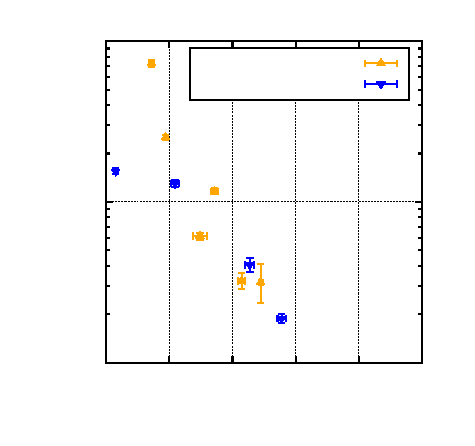
\includegraphics{ktaunonconf}}%
    \gplfronttext
  \end{picture}%
\endgroup

}}
\caption{Dispersionsrelation för strängarnas olika egenmoder. Bortsett från de moder med lägt $k$ så ser dispersionsrelationen ut att kunna vara exponeniell.
Felmariginalerna för $\tau$ är satta som 99\,\%-iga konfidensintervall; för $k$ är de bara uppskattade genom att undersöka hur anpassningen försämras om man ändrar $k$.
\\\textcolor{red}{\Large Till Robin: Vi måste ändra hur vi beräknar $\Delta{k}$. Som det är nu ger bättre anpassning större osäkerhet.}
}
\label{fig:ktau}
\end{figure}

%Resultat som kan tas med

%Motivera att jämviktsläge fanns
%Uppdelningen i egenmoder, olika relaxationstid
%Dispersionsrelation?
%Skillnad mellan confined och unconfined



\section{Diskussion}

Nedan finns förslag på rubriker, ändra gärna och lägg till

\subsection{Polynomanpassningens påverkan på resultatet}

\subsection{Strängen verkar vibrera kring ett jämviktläge}

\subsection{Skillnad mellan non-confined och confined}

\subsection{hur $L_{p}>>L_{sträng}$ påverkar resultaten}


%Bara en liten kodsnutt som behövs när man kompilerar lokalt
%%% Local Variables: 
%%% mode: latex
%%% TeX-master: "00main.tex"
%%% End: 